%------------------------------------------------------------------------------------------------------------------------
\chapter{試験結果データ管理システムの開発}
\label{sec:}
%------------------------------------------------------------------------------------------------------------------------

本研究では、これまで読み出し試験用に開発されていたシステムの他に、モジュールの品質管理の流れの全てをサポートできるように機能の作成を行った。本研究において開発した項目を以下に示す。
\begin{itemize}
  \item ピクセル検出器情報の登録
  \item 品質試験結果の閲覧
  \item 品質試験結果のアップロード
  \item 品質試験結果のダウンロード
\end{itemize}

%------------------------------------------------------------------------------------------------------------------------
\section{ピクセル検出器情報の登録}
\label{sec:register-module}
%------------------------------------------------------------------------------------------------------------------------


%------------------------------------------------------------------------------------------------------------------------
\subsection{ピクセル検出器情報の管理方法}
\label{sec:register-module}
%------------------------------------------------------------------------------------------------------------------------

\begin{figure}[tbp]
  \centering
  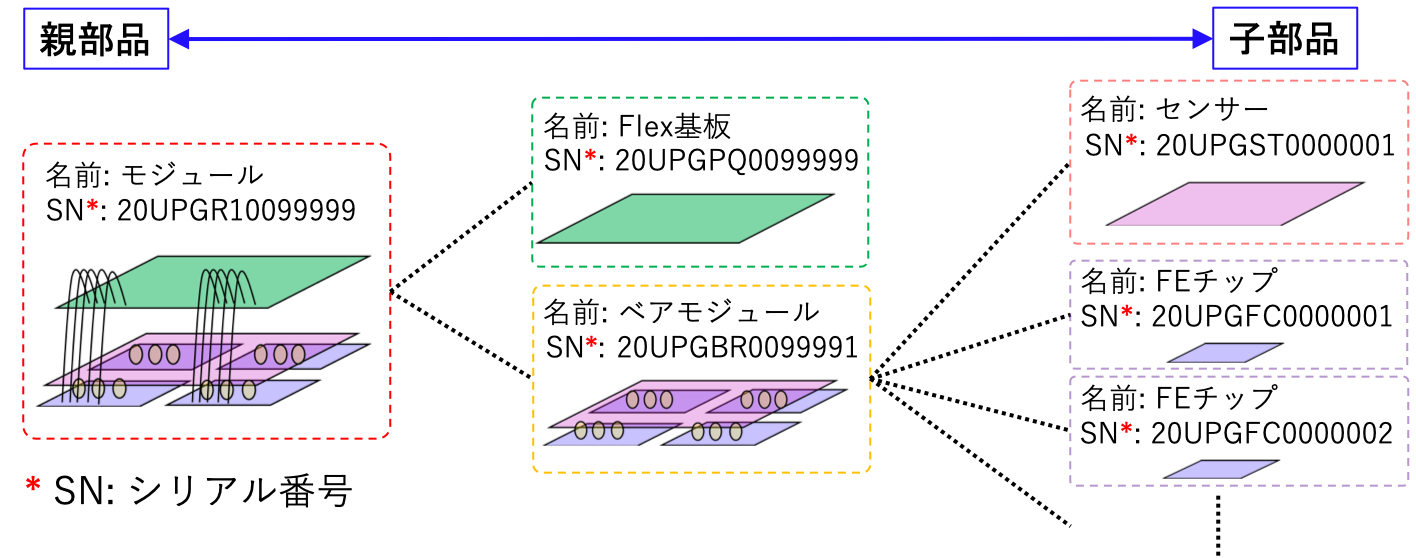
\includegraphics[height=6cm,keepaspectratio]{moduleCP.png}
  \caption[ピクセル検出器の親子関係]{ピクセル検出器の親子関係}
  \label{fig:moduleCP}
\end{figure}

%------------------------------------------------------------------------------------------------------------------------
\section{試験結果の管理}
\label{sec:show-nonelec}
%------------------------------------------------------------------------------------------------------------------------




%------------------------------------------------------------------------------------------------------------------------
\section{試験結果のアップロード}
\label{sec:upload-result}
%------------------------------------------------------------------------------------------------------------------------




%------------------------------------------------------------------------------------------------------------------------
\section{試験結果のダウンロード}
\label{sec:download-result}
%------------------------------------------------------------------------------------------------------------------------



%------------------------------------------------------------------------------------------------------------------------
\section{試験結果の評価}
\label{sec:elec-eval}
%------------------------------------------------------------------------------------------------------------------------





%------------------------------------------------------------------------------------------------------------------------
\section{本章のまとめ}
\label{sec:summary-7}
%------------------------------------------------------------------------------------------------------------------------



\newpage
